\section{Introduction}
\label{sec:intro}

With the rapid proliferation of social media, images are increasingly used to share daily experiences, emotions, and personal viewpoints. Visual intention recognition aims to infer the latent purpose conveyed by an image, and has become an important problem in human-centered multimedia analysis \cite{jia_intentonomy_2021, wen_dip_2023}, with applications ranging from user interest understanding to psychological and behavioral profiling and broader social media content analysis.

Compared with conventional image classification, which assigns images to relatively objective categories such as objects, scenes, or actions, intention recognition must map visual evidence to abstract and subjective intent labels. Such labels are rarely determined by local visual cues alone, and instead emerge from a holistic interpretation of scene context, human activities, object configurations, social interactions, and commonsense knowledge. The main difficulty therefore lies not in visual representation learning, but in bridging concrete image content and abstract intention semantics.

A central challenge of this task is its inherent ambiguity, which manifests in two distinct forms, as shown in Figure~\ref{fig:teaser}(a). The first is semantic ambiguity, since intent labels are often semantically adjacent, partially overlapping, or hierarchically correlated, so different labels may correspond to visually similar patterns while the same intent is expressed through diverse appearances, giving high inter-class similarity together with substantial intra-class variation. The second is supervisory ambiguity, since intention recognition is intrinsically subjective and different audiences may infer different yet plausible intentions from the same image, so the supervisory signal itself becomes unstable on samples with severe disagreement, and optimizing directly against hard labels forces the model to fit oversimplified targets and harms the robustness of the learned decision boundaries. Recent studies increasingly argue that such disagreement should be treated not as annotation noise but as meaningful uncertainty reflecting the structure of subjective interpretation itself \cite{peterson_human_2019, mostafazadeh_davani_dealing_2022}.

\begin{figure}[t]
\centering
\begin{subfigure}[t]{0.51\linewidth}
\centering
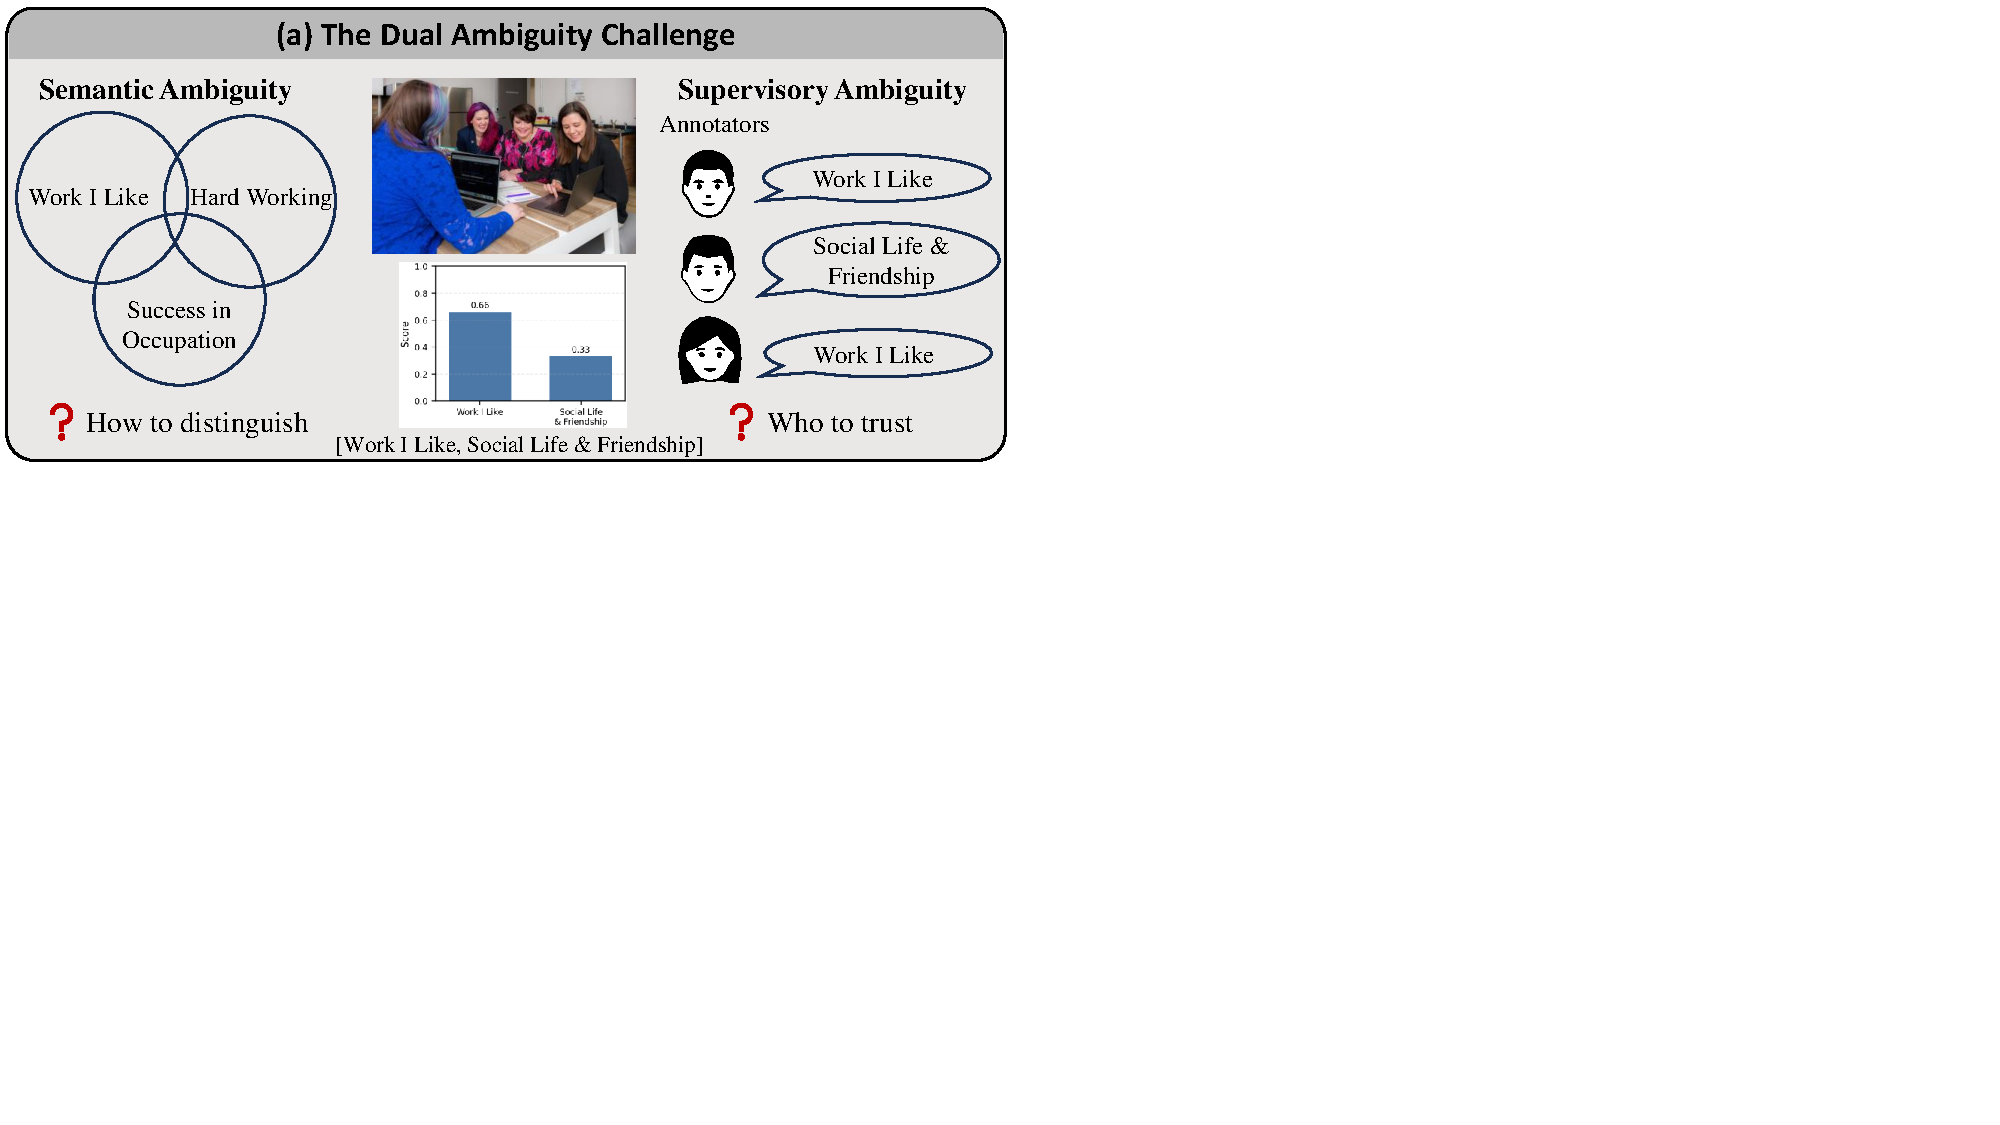
\includegraphics[width=\linewidth]{1_teaser_a.pdf}
\end{subfigure}
\hfill
\begin{subfigure}[t]{0.43\linewidth}
\centering
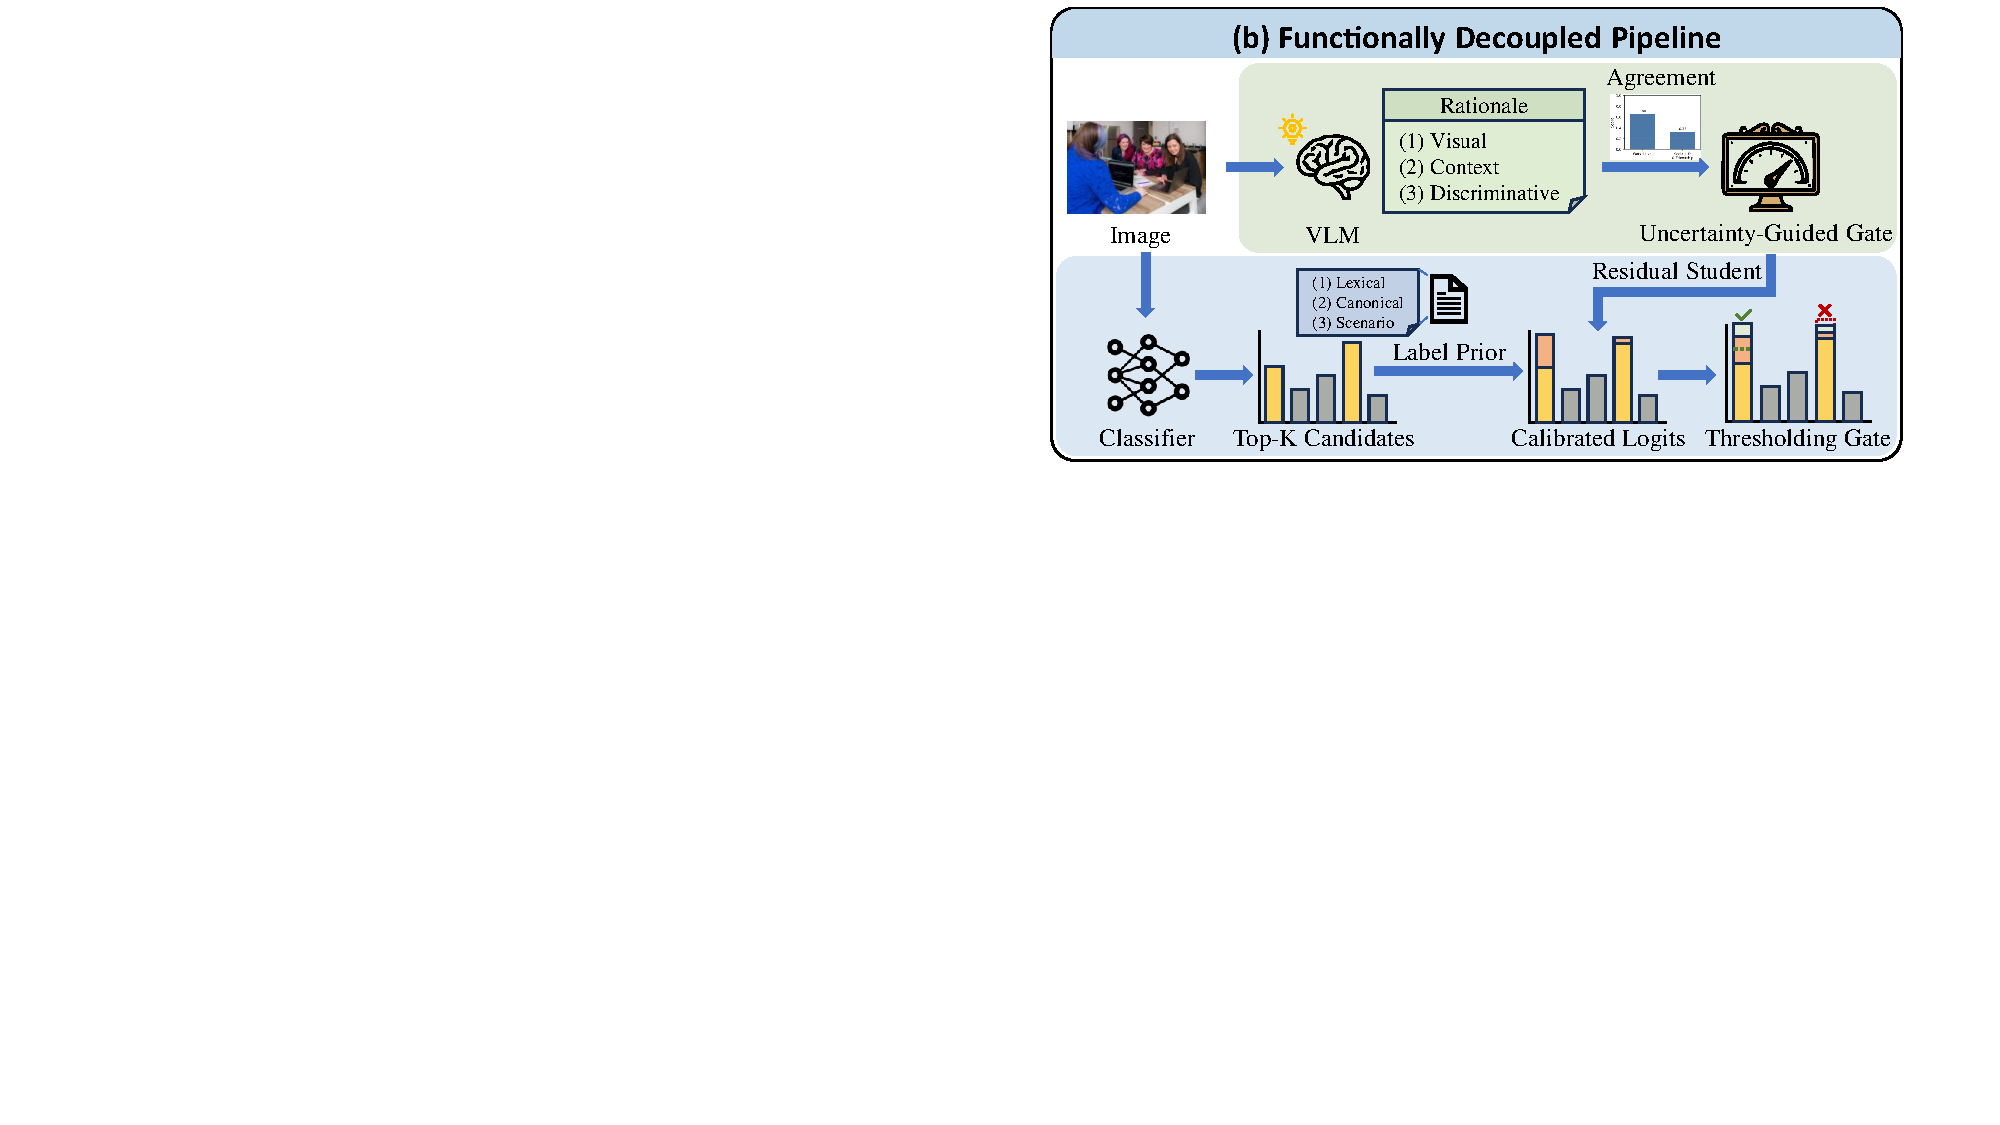
\includegraphics[width=\linewidth]{1_teaser_b.pdf}
\end{subfigure}
\caption{\textbf{Functionally decoupled ambiguity modeling in FDIL.} (a) Visual intent recognition suffers from semantic ambiguity among overlapping intents and supervisory ambiguity from annotator disagreement. (b) FDIL separates semantic refinement via Semantic Local Reranking and Calibration (SLR-C) from uncertainty-aware semantic supervision via Uncertainty-guided Text Distillation (UTD).}
\label{fig:teaser}
\end{figure}

Existing studies have attempted to alleviate these difficulties from different perspectives. 
Prototype-based methods, \textit{e.g.}, PIP-Net \cite{wang_prototype-based_2023}, introduce representative anchors to reduce feature-space confusion. 
Structure-aware methods, including CPAD \cite{ye_cross-modality_2023} and HLEG \cite{shi_learnable_2023}, exploit hierarchical label relationships to enhance multi-level semantic modeling and strengthen supervision. 
From the perspective of label quality, LabCR \cite{shi_label-aware_2024} explicitly models label shifting and label blemish to better cope with imperfect annotation distributions. 
More recently, knowledge-enhanced approaches have recognized that visual evidence alone is often insufficient for subjective intention understanding. 
IntCLIP \cite{leonardis_synergy_2025} incorporates the vision-language alignment knowledge of CLIP into the task, \revised{HVU-CLIP \cite{yang_holistic_2026} refines intent semantics iteratively and couples them with bidirectional visual-semantic interaction.} IntentMLM \cite{wang_unlocking_2026} further leverages multimodal large models, caption generation, and retrieval to perform more holistic intention perception\revised{, while CoT4Intent \cite{huang_cot4intent_2026} attributes the residual errors of MLLM-based intent classification to hallucination and suppresses it with structured chain-of-thought reasoning.} This line of work reflects a broader shift toward large vision-language and multimodal large language models (MLLMs) as sources of external semantic knowledge for subjective image understanding. However, our zero-shot experiments show that prompting a general-purpose MLLM directly remains below a task-trained model on this benchmark, since such models supply useful intent priors but not the dataset-specific calibration and uncertainty-aware supervision this task requires. Our purpose is therefore not to replace these models, but to convert their semantic knowledge into a structured prior and an uncertainty-gated training signal that explicitly target the two ambiguities below.

Although these methods have yielded encouraging progress, they typically treat one perspective of ambiguity as dominant. 
In our view, the core difficulty of subjective visual intention recognition is not any single ambiguity alone, but the coexistence of supervisory ambiguity and semantic ambiguity, which interfere with different functional components of the system. 
The former primarily corrupts supervision by compressing diverse subjective interpretations into rigid targets, whereas the latter primarily distorts local decision geometry by making neighboring labels difficult to separate. 
Treating these two failure modes within one mechanism may therefore be suboptimal, as it is difficult to simultaneously achieve robust learning on disagreement-prone samples and precise discrimination among closely related intents.

Motivated by this observation, we propose \textbf{FDIL} (\textbf{F}unctionally \textbf{D}ecoupled \textbf{I}ntent \textbf{L}earning), a functionally decoupled framework for subjective intent recognition, as illustrated in Figure~\ref{fig:teaser}(b), where fixed semantic priors provide structured candidate semantics, uncertainty-aware text teachers stabilize ambiguous supervision, and a residual student learns image-aware intent prediction on top of the semantic prior.
Ambiguity handling is decoupled into two complementary functions. Semantic Local Reranking and Calibration (SLR-C) provides ambiguity-aware semantic refinement, where heterogeneous lexical, canonical, and scenario priors define a semantic prior supplying structured candidate semantics. Uncertainty-guided Text Distillation (UTD) provides ambiguity-aware semantic supervision, where a text-only teacher distilled from rationale embeddings regularizes the visual model according to annotator agreement, improving robustness under subjective supervision and supporting image-aware prediction on top of the semantic prior. Together they improve robustness and discriminability without high architectural complexity.

Extensive experiments on the Intentonomy dataset show that FDIL outperforms baselines and recent state-of-the-art methods in both hard-sample robustness and overall multi-label prediction quality.
\revised{We further transfer FDIL to the larger EMOTIC benchmark and to the Flickr-LDL and Emotion6 label-distribution benchmarks, where the division of labour survives on a larger transfer benchmark and under a different prediction space.}

The main contributions of this work are summarized as follows:
\begin{itemize}
    \item We reformulate visual intention recognition as a \emph{functionally decoupled} ambiguity problem, treating supervisory ambiguity and semantic ambiguity as two separately justified functional roles rather than a single undifferentiated mechanism. This decomposition outperforms a strong unified alternative while keeping each function individually interpretable, separately measurable, and independently deployable.
    \item We propose Semantic Local Reranking and Calibration (SLR-C) together with residual semantic refinement, where heterogeneous textual priors first define a semantic prior with structured candidate semantics and a lightweight residual student further adapts prediction to image evidence.
    \item We propose Uncertainty-guided Text Distillation (UTD), which leverages annotator disagreement as an uncertainty signal to adaptively introduce semantic guidance, improving robustness under ambiguous supervision.
\end{itemize}
